\begin{frame}{Base de numération}
  \begin{itemize}
    \item On parle de \textit{base} ou \textit{radix} $r$.
    \begin{itemize}
      \item Utilisation des \textit{symboles} de $0$ à $r-1$.
      \item Notation \textit{positionnelle}
      \item Les entiers se décomposent à l'aide des coefficients des puissances de $r$.
    \end{itemize}

    \item Base 10 :
    \begin{itemize}
      \item $142 = 1\times 10^2 + 4 \times 10^1 + 2  \times 10^0$
    \end{itemize}

    \item Base 10, nombres décimaux :
    \begin{itemize}
      \item $142.34 = 1\times 10^2 + 4 \times 10^1 + 2  \times 10^0 + 3 \times 10^{-1} + 4 \times 10^{-2}$
      \item Nombre décimal $\frac{a}{10^n}$ $\rightarrow$ nombre fini de symboles.
      \item Attention : tous les nombres à virgule ne sont pas décimaux !
      \item Attention : lorsqu'on change de base, le nombre de coefficients nécessaires, pour une précision donnée, varie.
      \begin{itemize}
        \item Exemple : $0.2$ ne se représente pas avec un nombre fini de \texttt{bits} dans la base $2$ !
      \end{itemize}

    \end{itemize}
  \end{itemize}
\end{frame}

\begin{frame}{Notations non positionnelles : trois exemples}

\textbf{Chiffres romains} \hfill \textit{(additif, symboles à valeur fixe)}

\smallskip
I = 1, V = 5, X = 10, L = 50, C = 100, D = 500, M = 1000

\smallskip
Exemple : MCMXCIV = 1000 + (1000-100) + (100-10) + (5-1) = \textbf{1994}

\vspace{0.6cm}

\textbf{Système unaire} \hfill \textit{(additif pur, une marque par unité)}

\smallskip
\texttt{|||||} = 5 \qquad \texttt{|||||||} = 7 \quad \textit{(ou groupes de 5)}

\vspace{0.6cm}

\textbf{Hiéroglyphes égyptiens} \hfill \textit{(additif, un symbole par puissance de 10)}

\smallskip
\begin{tabular}{ll}
$\vert$ = 1 & $\cap$ = 10 \\
$\curlywedge$ = 100 & $\odot$ = 1000 \\
\end{tabular}

\smallskip
24 s'écrit : deux « anses » + quatre « traits » --- \textbf{l'ordre n'importe pas}

\vspace{0.4cm}

\centering
\footnotesize\itshape
Dans tous ces systèmes, la position d'un symbole ne modifie jamais sa valeur.

\end{frame}

\begin{frame}{Généralisation}
  La formule générale pour la base 10 est bien entendu :
  $$ x = \sum_{i=-\infty}^{i=+\infty} c_i.10^i, c_i \in \{0,\dots,9 \}$$
  et se généralise :
  $$ \forall r, x = \sum_{i=-\infty}^{i=+\infty} c_{i,r}.r^i, c_{i,r} \in \{0,\dots,(r-1)\}$$
  Lors des changements de base, il faut une notation pour préciser la base de représentation.
  \begin{itemize}
    \item Par exemple : $ 142_{10} = 10001110_{2}$
    \item En logiciel : $ 142_{10} = \text{\texttt{0b10001110}} = \text{\texttt{0x8e}} = \text{\texttt{0o216}}$

    \end{itemize}
\end{frame}

\begin{frame}{Compter en binaire : convertir par table}

  \begin{columns}
    \begin{column}{0.5\textwidth}
      \begin{table}[h]
        \centering
        \resizebox{!}{0.44\textheight}{%
        \begin{tabular}{c|ccccc}
          \toprule
          \multirow{2}{*}{\textbf{Decimal count}} & \multicolumn{5}{c}{\textbf{Binary count}} \\
          \cmidrule(l){2-6} & \textbf{16s} & \textbf{8s} & \textbf{4s} & \textbf{2s} & \textbf{1s} \\
          \midrule
          0  &   &   &   &   & 0 \\
          1  &   &   &   &   & 1 \\
          2  &   &   &   & 1 & 0 \\
          3  &   &   &   & 1 & 1 \\
          4  &   &   & 1 & 0 & 0 \\
          5  &   &   & 1 & 0 & 1 \\
          6  &   &   & 1 & 1 & 0 \\
          7  &   &   & 1 & 1 & 1 \\
          8  &   & 1 & 0 & 0 & 0 \\
          9  &   & 1 & 0 & 0 & 1 \\
          10 &   & 1 & 0 & 1 & 0 \\
          11 &   & 1 & 0 & 1 & 1 \\
          12 &   & 1 & 1 & 0 & 0 \\
          13 &   & 1 & 1 & 0 & 1 \\
          14 &   & 1 & 1 & 1 & 0 \\
          15 &   & 1 & 1 & 1 & 1 \\
          16 & 1 & 0 & 0 & 0 & 0 \\
          17 & 1 & 0 & 0 & 0 & 1 \\
          18 & 1 & 0 & 0 & 1 & 0 \\
          19 & 1 & 0 & 0 & 1 & 1 \\
          \midrule
          & $2^4$ & $2^3$ & $2^2$ & $2^1$ & $2^0$ \\
          \cmidrule(l){2-6}
          & \multicolumn{5}{c}{Powers of 2} \\
          \bottomrule
        \end{tabular}
        % \vspace{1pt}
        % \hspace{2.cm}\textbf{MSB} \hfill \textbf{LSB}\hspace{0.1cm}
        } %resizex
      \end{table}
    \end{column}

    \begin{column}{0.5\textwidth}
      \begin{table}[h]
      \centering
        \resizebox{!}{0.44\textheight}{
        \begin{tabular}{cccc}
        \toprule
        \textbf{Décimal} & \textbf{Binaire} & \textbf{Octal} & \textbf{Hexadécimal} \\
        \midrule
        0  & 0000 & 0  & 0 \\
        1  & 0001 & 1  & 1 \\
        2  & 0010 & 2  & 2 \\
        3  & 0011 & 3  & 3 \\
        4  & 0100 & 4  & 4 \\
        5  & 0101 & 5  & 5 \\
        6  & 0110 & 6  & 6 \\
        7  & 0111 & 7  & 7 \\
        8  & 1000 & 10 & 8 \\
        9  & 1001 & 11 & 9 \\
        10 & 1010 & 12 & A \\
        11 & 1011 & 13 & B \\
        12 & 1100 & 14 & C \\
        13 & 1101 & 15 & D \\
        14 & 1110 & 16 & E \\
        15 & 1111 & 17 & F \\
        \bottomrule
      \end{tabular}
      }
      \end{table}
    \end{column}

  \end{columns}
\end{frame}

\begin{frame}{A quoi ça sert ?}
  \begin{center}
    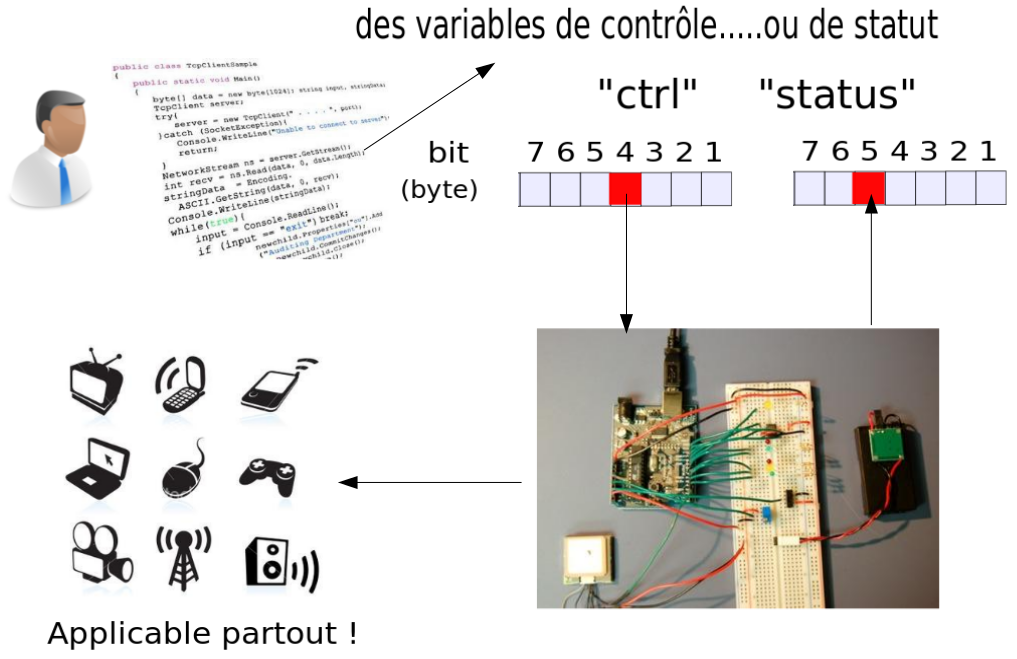
\includegraphics[scale=0.3]{./images/numbers_2.png}
  \end{center}
\end{frame}

\begin{frame}{A quoi ça sert ?}
  \begin{columns}
    \begin{column}{0.5\textwidth}
      \begin{center}
        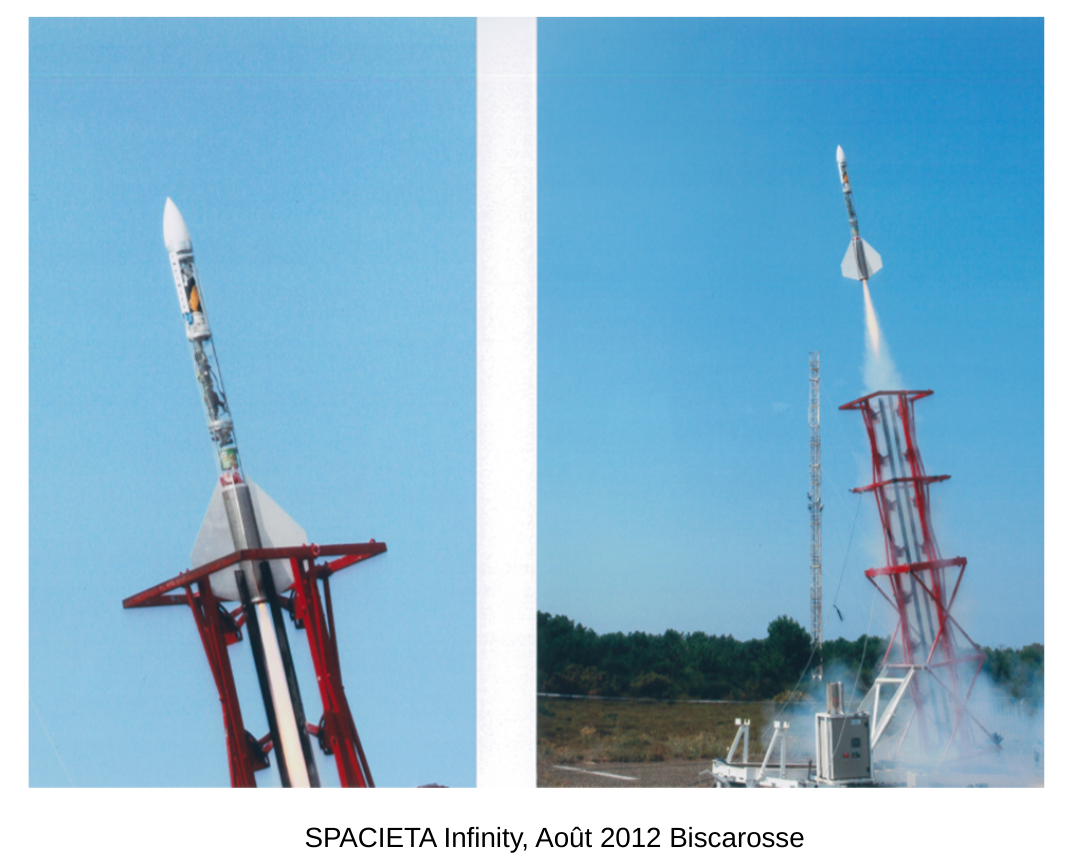
\includegraphics[scale=0.18]{./images/spacieta.png}
      \end{center}
    \end{column}

    \begin{column}{0.5\textwidth}
      \begin{center}
        \includegraphics[scale=0.18]{/home/jcll/Dropbox/IMAGES_TECHNIQUES/JOG.jpg}
      \end{center}
      JOG : conçu  à l'ENSTA Bretagne pour l'enseignement 1A.
    \end{column}
  \end{columns}
\end{frame}

\begin{frame}{Conversions entre bases : par table}
  \begin{center}
    \small $101101_{2} = \text{10\_1101}_{2} = \text{0010\_1101}_{2} = 2D_{16} = \mathbf{0x2D}$
  \end{center}

  \smallskip
  {\small Dans le cas de nombres fractionnaires, on rajoute des 0 à droite de la
  partie fractionnaire. Ainsi~:}

  \begin{center}
    \small le nombre $1011.01_{2} = \text{1011.0100}_{2} = B.4_{16}$
  \end{center}

  \smallskip
  {\small On procède de même pour la traduction octale.}

  \begin{center}
    \small $(10110001101011.1111)_{2} = (\text{101 110 001 101 011}.\text{111 100})_{2} = (36153.74)_{8}$
  \end{center}

  \smallskip
  \begin{center}
    \small
    \begin{tabular}{cccc}
      4 & 7 & . & F \quad E \\[-2pt]
      $\downarrow$ & $\downarrow$ & & $\downarrow$ \qquad $\downarrow$ \\[-2pt]
      0100 & 0111 & . & 1111 \quad 1110
    \end{tabular}

    \smallskip
    \small $47.\text{FE}_{16} \approx 1000111.1111111_{2}$
  \end{center}

\end{frame}

\begin{frame}{Conversions entre bases : par calcul}
  \begin{center}
    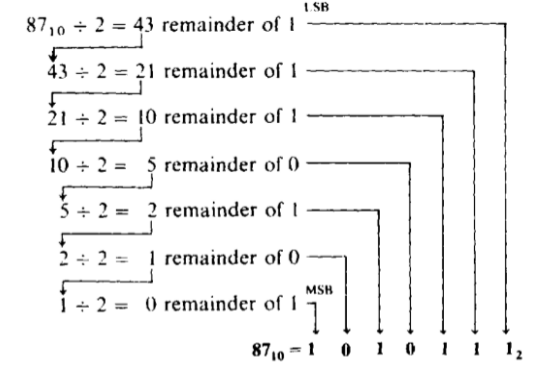
\includegraphics[scale=0.5]{./images/numbers_5.png}
  \end{center}
\end{frame}

\begin{frame}{Conversions entre bases : par calcul}
  \begin{center}
    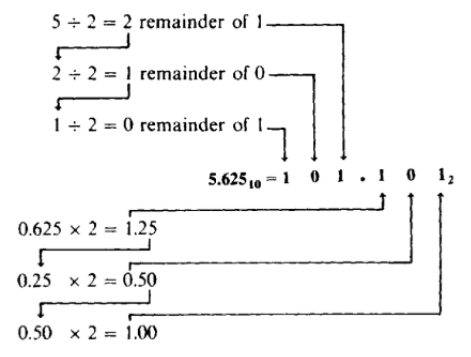
\includegraphics[scale=0.5]{./images/numbers_6.png}
  \end{center}
\end{frame}

\begin{frame}{Conversions entre bases : par calcul}
  \begin{center}
    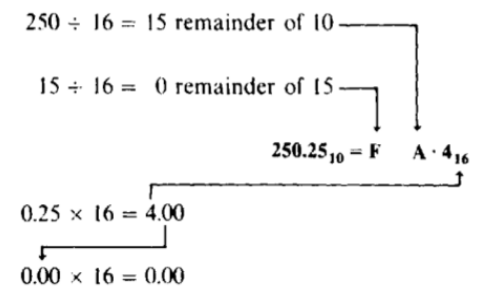
\includegraphics[scale=0.5]{./images/numbers_7.png}
  \end{center}
\end{frame}

\begin{frame}{Autres codes binaires : BCD décimal codé binaire}
  \begin{center}
    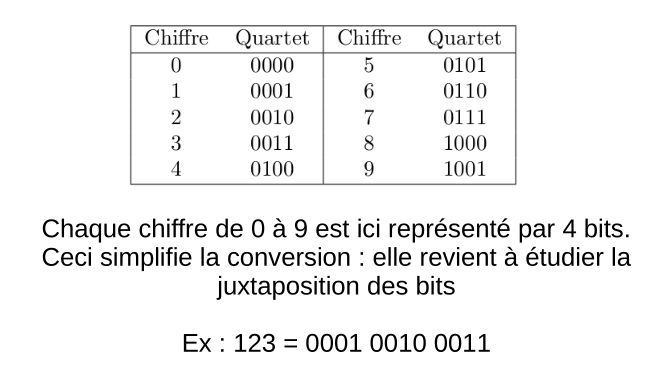
\includegraphics[scale=0.5]{./images/numbers_8.png}
  \end{center}
\end{frame}

\begin{frame}{Autres codes binaires : code de gray ou binaire réfléchi}
  \begin{center}
    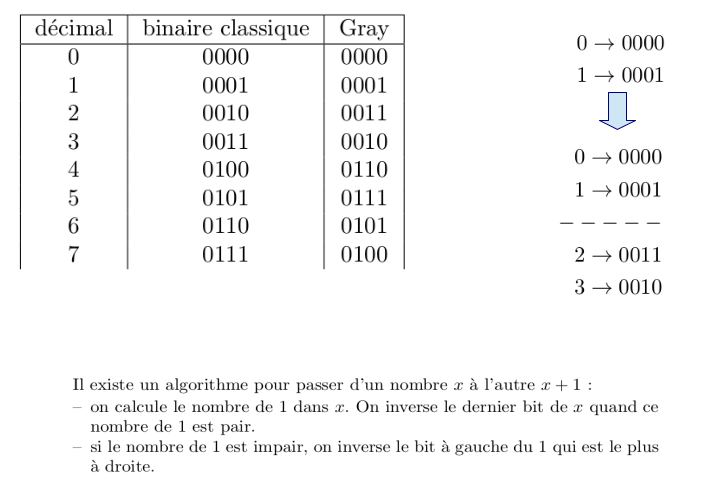
\includegraphics[scale=0.4]{./images/numbers_9.png}
  \end{center}
\end{frame}

\begin{frame}{Entiers positifs ou \texttt{unsigned}}
  \bigskip
  Soit un nombre $W$ de bits et soit $\vec{x} = [x_{w-1},x_{w-2},\ldots,x_0]$ de
  bits. Nous avons vu précédemment (sans la nommer) que la simple fonction~:
  \[
    B2U_w(\vec{x}) \doteq \sum_{i=0}^{w-1} x_i 2^i
  \]
  définit la valeur non-signée ("unsigned") de $\vec{x}$, dans $\mathbb{N}$.
  Les valeurs limites de cette fonction sont~:
  \[
    \begin{cases}
      UMax_w = \sum_{i=0}^{w-1} 2^i = 2^w - 1 \\
      UMmin_w = \sum_{i=0}^{w-1} 0 = 0
    \end{cases}
  \]
  On a donc~:
  \[
    B2U_w : \{0,1\}^w \to \{0,\ldots,2^w-1\}
  \]
\end{frame}

\begin{frame}{Complément à 2 sur w bits}
 \medskip
  \small
  De manière similaire, on définit désormais la fonction qui permet de
  calculer la valeur du vecteur $\vec{x}$ dans le cas d'une valeur signée,
  c'est-à-dire négative ou positive, \textbf{en complément à 2}.
  \[
    B2T_w(\vec{x}) \doteq -x_{w-1}2^{w-1} + \sum_{i=0}^{w-2} x_i 2^i
  \]
  Désormais, le bit de poids fort, le plus à gauche, contribue de manière
  négative à la somme totale. Précisons également que le 'T' vient de
  "two's complement". Calculons les valeurs min et max de cette fonction.
  Pour $\vec{x} = [10\ldots0]$ et $\vec{x} = [01\ldots1]$ respectivement, on
  trouve~:
  \[
    \begin{cases}
      TMin_w = -2^{w-1} \\
      TMax_w = \displaystyle\sum_{i=0}^{w-2} 2^i = 2^{w-1} - 1
    \end{cases}
  \]
  On a donc~:
  \[
    B2U_w : \{0,1\}^w \to \{-2^{w-1},\ldots,2^{w-1}-1\}
  \]
  On pourra également dénoter cette fonction $C_{2,w}(\vec{x})$.
\end{frame}

% ===================================================================
\begin{frame}{Complément à 2 sur w bits}

  \bigskip
  \begin{center}
    \renewcommand{\arraystretch}{1.15}
    \begin{tabular}{|c|c||c|}
      \hline
      \textbf{signé} & \textbf{bit vector} & \textbf{non-signé} \\
      \hline
      $-4$ & 100 & 4 \\ \hline
      $-3$ & 101 & 5 \\ \hline
      $-2$ & 110 & 6 \\ \hline
      $-1$ & 111 & 7 \\ \hline
      $0$  & 000 & 0 \\ \hline
      $1$  & 001 & 1 \\ \hline
      $2$  & 010 & 2 \\ \hline
      $3$  & 011 & 3 \\ \hline
    \end{tabular}
  \end{center}
\end{frame}

% ===================================================================
\begin{frame}{Nombres négatifs}

  \bigskip
  Le complément à 1 d'un nombre binaire consiste à simplement inverser tous
  ses bits.
  \medskip
  Le complément à 2 d'un nombre binaire s'obtient ainsi:
  \begin{itemize}
    \item On parcourt le nombre en partant de la droite (bit de poids faible).
    \item On recopie tel quel tous les bits tant qu'on n'a pas rencontré le premier 1.
    \item On recopie ce premier 1.
    \item On inverse tous les bits suivants (à gauche de ce 1).
  \end{itemize}
  Il existe toutefois une autre méthode, qui se retient plus facilement
  (peut-être). Elle consiste en une formule simple~:

  \bigskip
  \begin{columns}
    \begin{column}{0.35\textwidth}
      \colorbox{blue!20}{\parbox{0.9\textwidth}{\small\textbf{Attention~!!!!}\\
      $-134$ nécessite 9 bits et non 8}}
    \end{column}
    \begin{column}{0.65\textwidth}
      \begin{tikzpicture}
        \node[draw, fill=gray!30, minimum width=3cm, minimum height=1cm, font=\Large] (box) {$-X = \overline{X} + 1$};
        \node[below=0.9cm of box, align=left, xshift=0.3cm] (lab) {\footnotesize Addition classique\\\footnotesize (et non « OU » binaire)};
        \draw[-{Latex[length=3mm]}] (lab.north -| box.south) -- (box.south);
      \end{tikzpicture}
    \end{column}
  \end{columns}
\end{frame}

% ===================================================================
\begin{frame}{Nombres négatifs : représentations obsolètes}
  \bigskip
  \small
  La représentation en magnitude signée est simplement~:
  \[
    B2S_w(\vec{x}) \doteq (-1)^{x_{w-1}} \sum_{i=0}^{w-2} x_i 2^i
  \]
  Il existe également une représentation des nombres en complément à 1,
  très légèrement différente du complément à 2.
  \[
    B2T_w(\vec{x}) \doteq -x_{w-1}(2^{w-1}-1) + \sum_{i=0}^{w-2} x_i 2^i
  \]

  \bigskip
  \begin{center}
    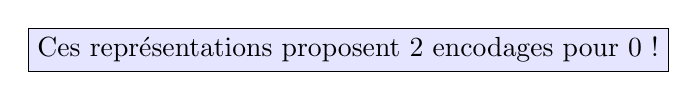
\begin{tikzpicture}
      %\node[arrow, fill=red, minimum height=1cm, arrow head extend=2mm] (arr) {};
      \node[draw, fill=blue!10, align=center] {Ces représentations proposent 2 encodages pour 0~!};
    \end{tikzpicture}
  \end{center}

  \normalsize
  Dans le cas de la magnitude signée~:\\
  $+0 = 0\ldots.0$ et $-0 = 10\ldots0$
\end{frame}

% ===================================================================
\begin{frame}{Nombres négatifs : résumé}
  \begin{columns}[t]
    \begin{column}{0.42\textwidth}
      \tiny
      \renewcommand{\arraystretch}{1.05}
      \begin{tabular}{|c|c|}
        \hline
        \textbf{Signed decimal} & \textbf{8-bit 2's compl.} \\
        \hline
        $+127$ & 0111 1111 \\
        $+126$ & 0111 1110 \\
        $+125$ & 0111 1101 \\
        $\vdots$ & $\vdots$ \\
        $+1$ & 0000 0001 \\
        $+0$ & 0000 0000 \\
        \hline
        $-1$ & 1111 1111 \\
        $-2$ & 1111 1110 \\
        $\vdots$ & $\vdots$ \\
        $-125$ & 1000 0011 \\
        $-126$ & 1000 0010 \\
        $-127$ & 1000 0001 \\
        $-128$ & 1000 0000 \\
        \hline
      \end{tabular}
    \end{column}
    \begin{column}{0.58\textwidth}
      \small
      \begin{center}
        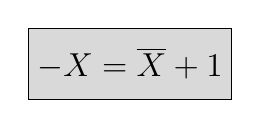
\begin{tikzpicture}
          \node[draw, fill=gray!30, minimum width=2.5cm, minimum height=0.9cm, font=\large] {$-X = \overline{X} + 1$};
        \end{tikzpicture}
      \end{center}

      \bigskip
      \colorbox{orange!40}{
      \begin{minipage}{0.95\textwidth}
        $-125\; ? =$

        \medskip
        $125 \quad = \quad 111\,1101$

        \medskip
        $/125 \quad = \quad \textcolor{red}{1}\,000\,0010$

        \medskip
        $/125+1 = 1\,000\,0011$
      \end{minipage}}
    \end{column}
  \end{columns}

  \bigskip
  \small
  Noter que les nombres en complément à 2 sont négatifs s'ils présentent un
  MSB à 1~!\\
  125 se représente sur 7 bits, mais pas $-125$~: il faut 8 bits
\end{frame}

% ===================================================================
\begin{frame}{\LARGE Exemple~: $-3$ sur 3 bits}


  \begin{columns}[t]
    \begin{column}{0.62\textwidth}
      \begin{itemize}
        \item $3_{10} = 011_2$
        \item $-3_{10} = /3_{10} + 1 = 100_2 + 1 = 101_2 = 5_{10}$~????
        \begin{itemize}
          \item 5 ne peut pas être représenté sur 3 bits, si on y
            représente également les nombres négatifs.
        \end{itemize}
      \end{itemize}

      \bigskip
      \colorbox{blue!30}{\parbox{0.95\textwidth}{\centering
        Pour un nombre donné de bits,\\
        il faut s'entendre sur le fait\\
        que la représentation d'un nombre est signée ou non}}
    \end{column}
    \begin{column}{0.35\textwidth}
      \small
      \begin{tabular}{cc}
        $+3$ & 011 \\
        $+2$ & 010 \\
        $+1$ & 001 \\
        $+0$ & 000 \\
        $-1$ & 111 \\
        $-2$ & 110 \\
        $-3$ & 101 \\
        $-4$ & 100 \\
      \end{tabular}
    \end{column}
  \end{columns}
\end{frame}

% ===================================================================
\begin{frame}{Addition et soustraction}

  \bigskip
  \textbf{Addition}~: classique
  \hfill
  \begin{minipage}{0.55\textwidth}
    \centering
    \renewcommand{\arraystretch}{1.2}
    \begin{tabular}{|l|r|}
      \hline
      & \textbf{Addition} \\
      \hline
      calcul & \begin{tabular}{r}0110\\ $+$0011\end{tabular} \\
      \hline
      retenus & 11 \\
      \hline
      résultat & 1001 \\
      \hline
    \end{tabular}
  \end{minipage}

  \bigskip
  \textbf{Soustraction : x - y}

  \small
  \begin{enumerate}
    \item on additionne $x$ et le complément à 2 de $y$
    \item si le résultat présente une retenue finale, on l'oublie~!
    \item s'il n'y a pas de retenue finale, on prend le complément à 2 du
      résultat et on place un signe "-" devant le nombre.
  \end{enumerate}

  \medskip
  \textbf{exemple}~: $x = 1101100_2$ et $y = 1011011_2$
  \[
    1101100 + 0100101 = 1\,0010001
  \]
  Le résultat est donc $x - y = 0010001_2$

  \hfill\tiny 108-91
\end{frame}

% ===================================================================
\begin{frame}{\LARGE Nombre en virgule fixe : ou \textit{fixed point}}

  \bigskip
  \begin{itemize}
    \item Déjà vu précédemment\ldots
    \item Le calculateur numérique devra connaître la position de la
      virgule, fixée une bonne fois pour toute.
    \item Impact sur les opérations classiques~:
    \begin{itemize}
      \item Le résultat de l'addition hérite de la position de la virgule
        identique à celle dans les opérandes
      \item Cela est changé pour les autres opérations.
    \end{itemize}
  \end{itemize}
\end{frame}

% ===================================================================
\begin{frame}{Nombres en virgule flottante : norme \texttt{ieee754}}

  \begin{center}
    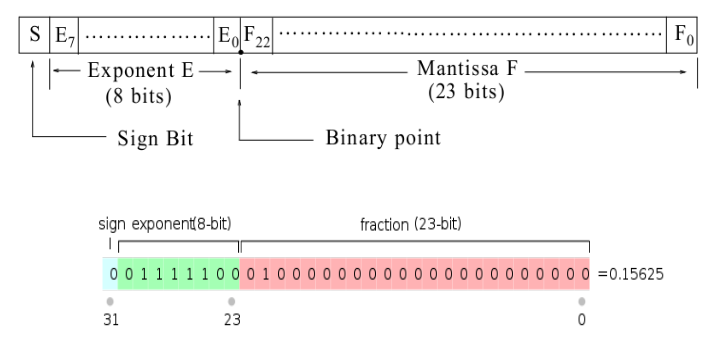
\includegraphics[scale=0.5]{./images/ieee754.png}
  \end{center}

  \bigskip
  \begin{center}
    \begin{tikzpicture}
      \node[single arrow, fill=blue!60, minimum height=1cm, single arrow head extend=2mm] (arr) {};
      \node[draw, fill=blue!10, right=0.2cm of arr] {Exo~: calculer le nombre max et min représentable};
    \end{tikzpicture}
  \end{center}
\end{frame}

% ===================================================================
\begin{frame}{IEEE 754 (SP)}
  \bigskip
  \begin{itemize}
    \item L'exposant est biaisé (en excédent) à 127. C'est-à-dire que pour
      coder un exposant $e$, on code le nombre $e+127$.
    \item Les exposants représentables vont de $-126$ à $127$ (les valeurs
      $00000000$ et $11111111$ sont réservées pour des cas exceptionnels)
    \item Les nombres sont normalisés, c'est-à-dire que la mantisse est
      entre 1 et 2.
  \end{itemize}
\end{frame}

% ===================================================================
\begin{frame}{IEEE 754 : cas exceptionnels}
  \bigskip
  \begin{itemize}
    \item Si $e = 11111111_2$ et $m=0$, le nombre représenté est $+$ ou $-$
      l'infini. Les opérations sur l'infini sont gérées correctement.
    \item Si $e = 11111111_2$ et $m \neq 0$, la représentation est
      considérée comme n'étant pas un nombre (NaN~: Not a Number).
    \item Si $e=0$ et $m=0$ on représente le nombre $+0$ ou $-0$ selon le
      signe.
    \item Si $e=0$ et $m \neq 0$ on dit que le nombre est dénormalisé.
      C'est-à-dire que la mantisse est écrite sans le 1 implicite.
  \end{itemize}
\end{frame}

% ===============================================================
\begin{frame}{Exemple de conversion  vers \texttt{ieee 754}}

  \textbf{Nombre à encoder :} $-12{,}375$

  \vspace{0.3cm}
  \textbf{1. Signe} \; : le nombre est négatif $\Rightarrow s = 1$

  \vspace{0.3cm}
  \textbf{2. Partie entière} \; : $12 = 1100_2$

  \vspace{0.3cm}
  \textbf{3. Partie fractionnaire} \; : $0{,}375$
  \[
    0{,}375 \times 2 = 0{,}75 \rightarrow 0 \qquad
    0{,}75 \times 2 = 1{,}5 \rightarrow 1 \qquad
    0{,}5 \times 2 = 1{,}0 \rightarrow 1
  \]
  \[
    \Rightarrow\; 12{,}375 = 1100{,}011_2
  \]

  \vspace{0.3cm}
  \textbf{4. Normalisation} \; : $\;1100{,}011_2 = 1{,}100011_2 \times 2^{3}$
  \begin{itemize}
    \item Mantisse : $m = 100011$
    \item Exposant réel : $e = 3$
    \item Exposant biaisé : $E = 3 + 127 = 130 = 10000010_2$
  \end{itemize}
\end{frame}

% ===============================================================
\begin{frame}{Étape 3 : assemblage des 32 bits}

  \begin{center}
  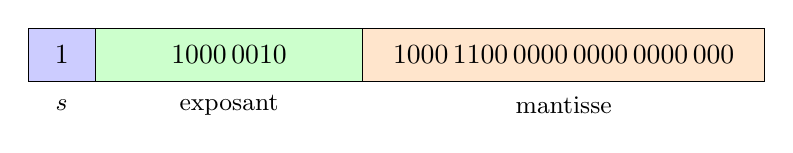
\begin{tikzpicture}[scale=0.85]
    \draw[fill=blue!20] (0,0) rectangle (1,0.8);
    \node at (0.5,0.4) {1};

    \draw[fill=green!20] (1,0) rectangle (5,0.8);
    \node at (3,0.4) {1000\,0010};

    \draw[fill=orange!20] (5,0) rectangle (11,0.8);
    \node at (8,0.4) {1000\,1100\,0000\,0000\,0000\,000};

    \node at (0.5,-0.35) {\small $s$};
    \node at (3,-0.35)   {\small exposant};
    \node at (8,-0.35)   {\small mantisse};
  \end{tikzpicture}
  \end{center}

  \vspace{0.4cm}
  \begin{block}{Résultat final}
    \[
      -12{,}375 \;\longrightarrow\;
      \underbrace{1}_{\text{signe}}\;
      \underbrace{10000010}_{\text{exposant}}\;
      \underbrace{10001100000000000000000}_{\text{mantisse}}
    \]
    \[
      \boxed{\texttt{0xC1460000}} \quad \text{(hexadécimal)}
    \]
  \end{block}

  \vspace{0.3cm}
  \textbf{Vérification :} $(-1)^1 \times 1{,}100011_2 \times 2^{130-127} = -12{,}375$ \checkmark
\end{frame}

\begin{frame}{\texttt{IEEE 754} : l'addition n'est pas commutative !}
  \begin{alertblock}{Avertissement}
    En arithmétique flottante IEEE 754, à cause des \textbf{arrondis},
    l'addition \textbf{n'est pas associative}, et dans certains cas elle
    peut même sembler \textbf{non commutative} lorsqu'on enchaîne
    plusieurs opérations ou qu'on change l'ordre des termes.
  \end{alertblock}

  \vspace{0.4cm}
  \textbf{Cause principale :} quand on additionne deux nombres d'ordres
  de grandeur très différents, le plus petit peut être \emph{entièrement
  absorbé} par l'arrondi du plus grand (\emph{absorption} / \emph{swamping}).

  \vspace{0.4cm}
  \begin{block}{Exemple classique en double précision}
    \[
      a = 1{,}0 \qquad b = 2^{-53} \qquad c = 2^{-53}
    \]
    \[
      (a + b) + c \;\neq\; a + (b + c)
    \]
  \end{block}

  \vspace{0.3cm}
  \centering
  \textit{L'ordre des opérations change le résultat !}
\end{frame}
\begin{frame}{Comment s'additionne-t-on deux flottants ?}
  \textbf{Algorithme matériel} (simplifié) pour $x + y$ :

  \vspace{0.4cm}
  \begin{enumerate}
    \item \textbf{Aligner les exposants} : on réécrit le plus petit
      exposant pour qu'il coïncide avec le plus grand. Les bits de sa
      mantisse sont \textbf{décalés vers la droite} — et les bits qui
      « sortent » sont \textbf{perdus}.
    \item \textbf{Additionner les mantisses} (avec le bit implicite).
    \item \textbf{Renormaliser} le résultat si nécessaire.
    \item \textbf{Arrondir} au format (au pair, par défaut).
  \end{enumerate}

  \vspace{0.4cm}
  \begin{block}{Le point critique}
    C'est à l'étape \textbf{1} que se joue tout le drame :
    si les exposants diffèrent de plus de $p$ bits (où $p$ est la
    précision), le plus petit nombre est \textbf{totalement
    sacrifié} au profit du plus grand.
  \end{block}

  % \vspace{0.2cm}
  % \centering
  % \begin{tikzpicture}[scale=0.9, every node/.style={font=\small}]
  %   \node[draw, rounded corners, fill=blue!10, inner sep=6pt] (x)
  %     {$x = 1{,}000\ldots0 \times 2^{0}$};
  %   \node[draw, rounded corners, fill=orange!10, inner sep=6pt,
  %         right=2cm of x] (y)
  %     {$y = 1{,}000\ldots0 \times 2^{-53}$};
  %   \draw[->, thick] (y.south) to[bend right=25]
  %     node[below, font=\scriptsize]{décalage de 53 bits vers la droite}
  %     (x.south);
  % \end{tikzpicture}
\end{frame}

% ===============================================================
\begin{frame}{\texttt{IEEE 754} : Illustration numérique}

  \textbf{Hypothèses :} double précision, $\varepsilon_{\text{mach}} = 2^{-52}$.
  Le plus petit incrément représentable autour de $1{,}0$ est
  $\text{ulp}(1) = 2^{-52}$.

  \vspace{0.4cm}
  \begin{columns}[T]
    \begin{column}{0.48\textwidth}
      \begin{block}{Calcul de $(a+b)+c$}
        \[
          a + b = 1{,}0 + 2^{-53}
        \]
        Or $2^{-53} = \tfrac{1}{2}\,\text{ulp}(1)$, donc l'arrondi
        (au pair) donne :
        \[
          a + b = 1{,}0
        \]
        Puis :
        \[
          (a+b) + c = 1{,}0
        \]
      \end{block}
    \end{column}

    \begin{column}{0.48\textwidth}
      \begin{block}{Calcul de $a+(b+c)$}
        \[
          b + c = 2^{-53} + 2^{-53} = 2^{-52}
        \]
        Cet incrément vaut exactement $\text{ulp}(1)$, donc il est
        représentable :
        \[
          a + (b+c) = 1{,}0 + 2^{-52}
        \]
      \end{block}
    \end{column}
  \end{columns}

  \vspace{0.2cm}
  \begin{center}
    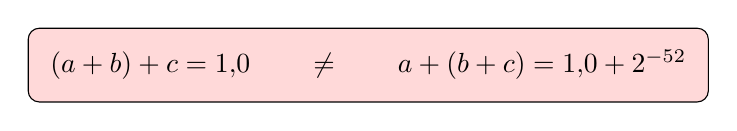
\begin{tikzpicture}
      \node[draw, rounded corners, fill=red!15, inner sep=8pt] {
        $(a+b)+c = 1{,}0 \qquad \neq \qquad a+(b+c) = 1{,}0 + 2^{-52}$
      };
    \end{tikzpicture}
  \end{center}

  \vspace{0.3cm}
  \begin{alertblock}{À retenir}
    Ne jamais tester l'égalité de deux calculs flottants pour une prise de décision.
  \end{alertblock}
\end{frame}


\begin{frame}{Douglas Hofstadter et les « faux » nombres réels}

  \begin{columns}[c]
    \begin{column}{0.28\textwidth}
      \centering
      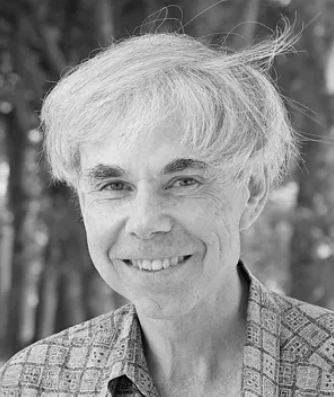
\includegraphics[scale=0.3]{./images/hofstadter.png}

      \vspace{0.2cm}
      {\scriptsize
        Douglas Hofstadter (1945--)\\
        \textit{Gödel, Escher, Bach}\\
        Prix Pulitzer 1980
      }
    \end{column}

    \begin{column}{0.70\textwidth}
      \begin{block}{}
        \itshape
        « En informatique, il n'y a pas de nombres réels. Il n'y a que
        des nombres flottants, et ils sont à peu près aussi réels que
        les personnages de dessins animés. »
      \end{block}

      \vspace{0.3cm}
      \small
      IEEE 754 ne code qu'un \textbf{ensemble fini} de valeurs, et
      chaque opération introduit un \textbf{arrondi}. Pourtant, cette
      arithmétique approximative pilote avions, réacteurs et ponts :
      la fiabilité vient des \textbf{algorithmes}, pas des nombres.
    \end{column}
  \end{columns}
\end{frame}

%============================================================================
\begin{frame}{Représentation des données symboliques}
  Certaines données ne sont pas numériques
  \begin{itemize}
    \item Enumérations, collections : couleurs,alphabets,...
    \item Ou compositions de données numériques
  \end{itemize}
Un encodage de ces données est nécessaire.
  \begin{center}
    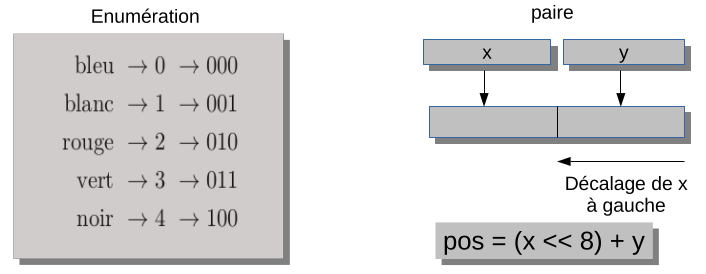
\includegraphics[scale=0.5]{./images/symb_0.png}
  \end{center}
\end{frame}

\begin{frame}{Représentation des données : codes \texttt{ASCII}}
  \begin{center}
    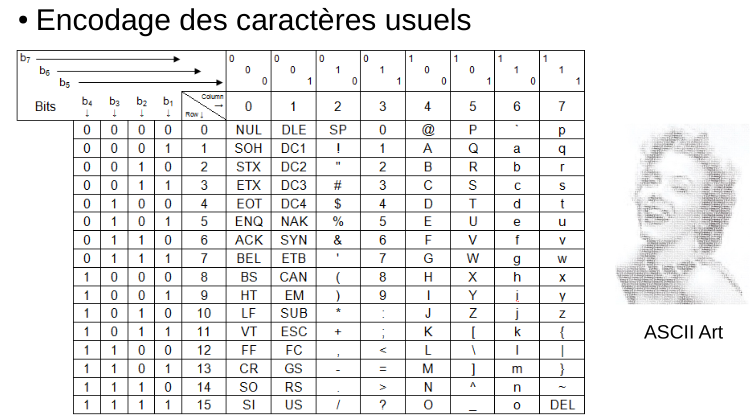
\includegraphics[scale=0.5]{./images/symb_1.png}
  \end{center}
\end{frame}

\begin{frame}{Représentation des données : codes \texttt{UTF8}}
  \begin{center}
    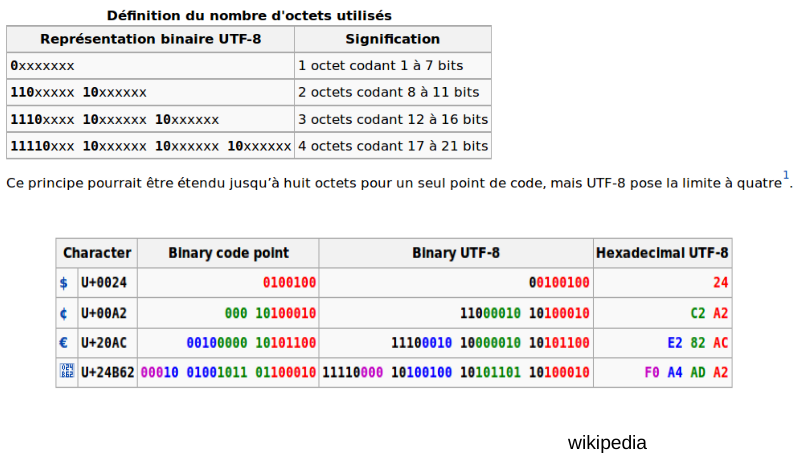
\includegraphics[scale=0.5]{./images/symb_2.png}
  \end{center}
\end{frame}

\begin{frame}{Manipulations binaires \textit{bitwise} : exemple}
  \begin{center}
    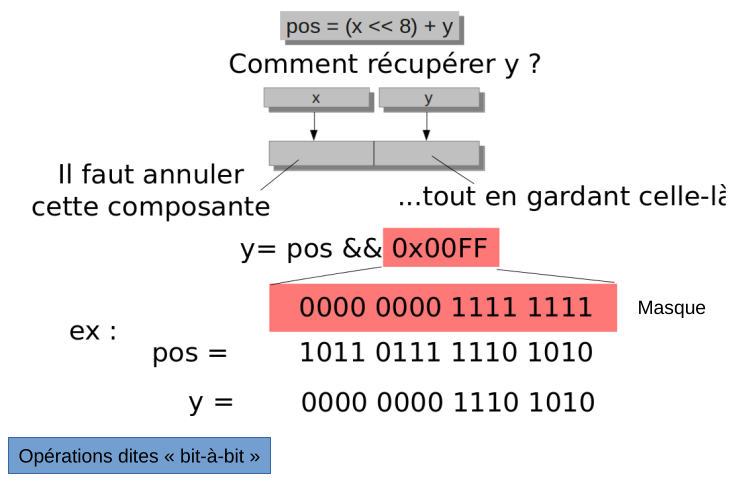
\includegraphics[scale=0.5]{./images/symb_4.png}
  \end{center}
\end{frame}

\begin{frame}{Manipulations binaires \textit{bitwise} traditionnelles}
  \begin{center}
    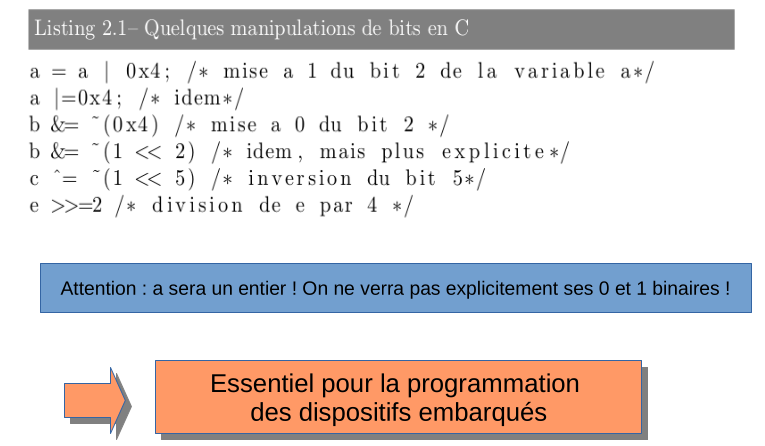
\includegraphics[scale=0.4]{./images/symb_6.png}
  \end{center}
\end{frame}

\begin{frame}{Codes détecteurs d'erreurs}
  \begin{center}
    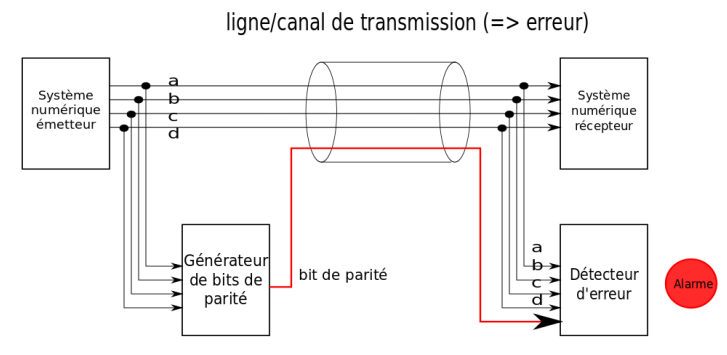
\includegraphics[scale=0.5]{./images/symb_7.png}
  \end{center}
\end{frame}

\begin{frame}{Codes détecteurs d'erreurs}
  \begin{center}
    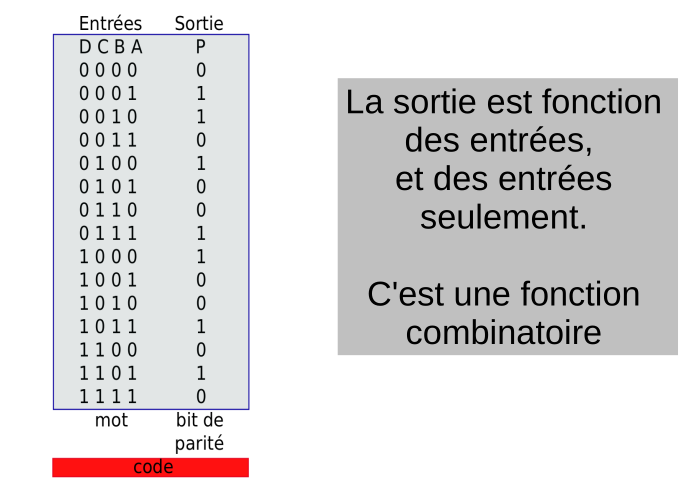
\includegraphics[scale=0.4]{./images/symb_8.png}
  \end{center}
\end{frame}

\begin{frame}{Claude Berrou et les turbocodes : correcteurs d'erreurs}

  \begin{columns}[c]
    \begin{column}{0.68\textwidth}
      \begin{block}{Une révolution née à Brest }
        \itshape
        En 1993, Claude Berrou et Alain Glavieux (ENST/IMT Atlantique) bouleversent la théorie
        de l'information en s'approchant de la \textbf{limite de Shannon},
        que les experts jugeaient inatteignable depuis 1948.
      \end{block}

      \vspace{0.3cm}
      \small
      Les \textbf{turbocodes} reposent sur un principe itératif :
      deux décodeurs élémentaires s'échangent des « croyances »
      jusqu'à converger vers le message original.

      \vspace{0.3cm}
      \textbf{Aujourd'hui :} 3G/4G, WiMAX, sondes spatiales
      (Mars Reconnaissance Orbiter, Messenger), plus de
      \textbf{4 milliards} de turbodécodeurs en circulation.
    \end{column}

    \begin{column}{0.28\textwidth}
      \centering
      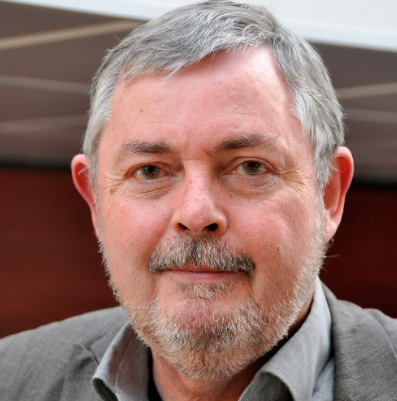
\includegraphics[scale=0.25]{./images/berrou.png}
      \vspace{0.2cm}
      {\scriptsize
        Claude Berrou (1951--)\\
        Télécom Bretagne\\
        Prix Marconi 2005\\
        Médaille Hamming 2003
      }
    \end{column}
  \end{columns}

\end{frame}
